

\documentclass[a4paper,12pt]{article}

\usepackage{amsmath}
\usepackage{amssymb}
\usepackage{amsfonts}
\usepackage{authblk}
\usepackage{bookmark}
\usepackage[makeroom]{cancel}
\usepackage{enumerate}
\usepackage{etoolbox}
\usepackage[left=2cm,right=2cm,top=2cm,bottom=2cm, nohead]{geometry}
\usepackage[pdftex]{graphicx}
\usepackage{hyperref}
\usepackage{natbib}
\usepackage{pdfpages}
\usepackage{subcaption}
\usepackage{tabularx} 
\usepackage{txfonts}
\usepackage{upgreek}
\usepackage{url}
\usepackage{xcolor}
\usepackage{ragged2e}
\usepackage[left=2cm,right=2cm,top=2cm,bottom=2cm]{geometry}

%\newcommand{\question}[2]{\textbf{\textit{#1}}\quad{\footnotesize\textit{(#2 points)}}\\[3mm]}
\newcommand{\question}[1]{\textbf{\textit{#1}}}
\newcommand{\points}[1]{\quad{\footnotesize\textit{(#1 points)}}}
\newcommand{\point}{\quad{\footnotesize\textit{(1 point)}}}
\newcommand{\HRule}{\rule{\linewidth}{0.3mm}}
\newcommand{\dd}{\mathrm{d}}
\renewcommand{\pi}{\uppi}
\newcommand{\ii}{\mathrm{i}}
\renewcommand{\thefootnote}{\normalsize\fnsymbol{footnote}}
\DeclareMathOperator{\e}{e}

\renewcommand{\theequation}{\Roman{equation}}

\begin{document}
\pagestyle{empty}

\begin{center}
\LARGE \textbf{Astronomy from 4 Perspectives: the Dark Universe}
\HRule
\end{center}
\begin{flushright}
prepared by: Jena participants
\end{flushright}
\begin{center}
{\Large \textbf{Questions: Dark matter and galaxy rotation curves}}
\end{center}
\vspace{5mm}



\begin{enumerate}[\itshape \bfseries 1.]
\item \question{Orientations of galaxies}\\
Think about how the galaxy should be orientated to be observed?\\
Here are some pictures as example:
\begin{figure}[h!]
	\centering
	\begin{subfigure}[t]{0.3\textwidth}
	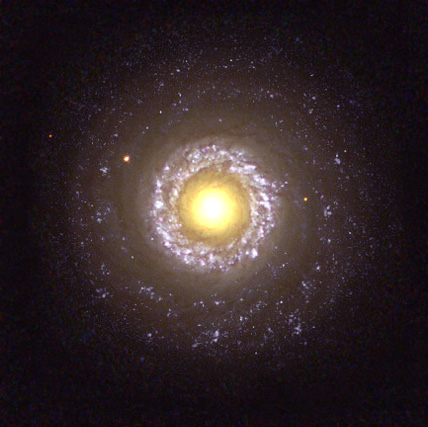
\includegraphics[height=5cm]{figures/gal1.jpg}
	\caption{Edge on galaxy NGC 7742\\Inclination angle $i =0^\circ$\\Image credit:\\Hubble Heritage Team\\(AURA/STScI/NASA/ESA)}
	\end{subfigure}
	\begin{subfigure}[t]{0.3\textwidth}
	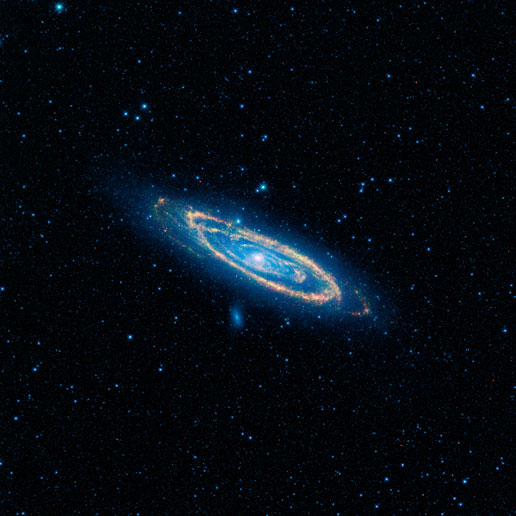
\includegraphics[height=5cm]{figures/gal2.jpg}
	\caption{Our galactic neighbour Andromeda as seen in infrared.\\
	Inclination angle $i \approx 13^\circ$\\Image credit:\\NASA/JPL-Caltech/UCLA}
	\end{subfigure}
	\begin{subfigure}[t]{0.3\textwidth}
	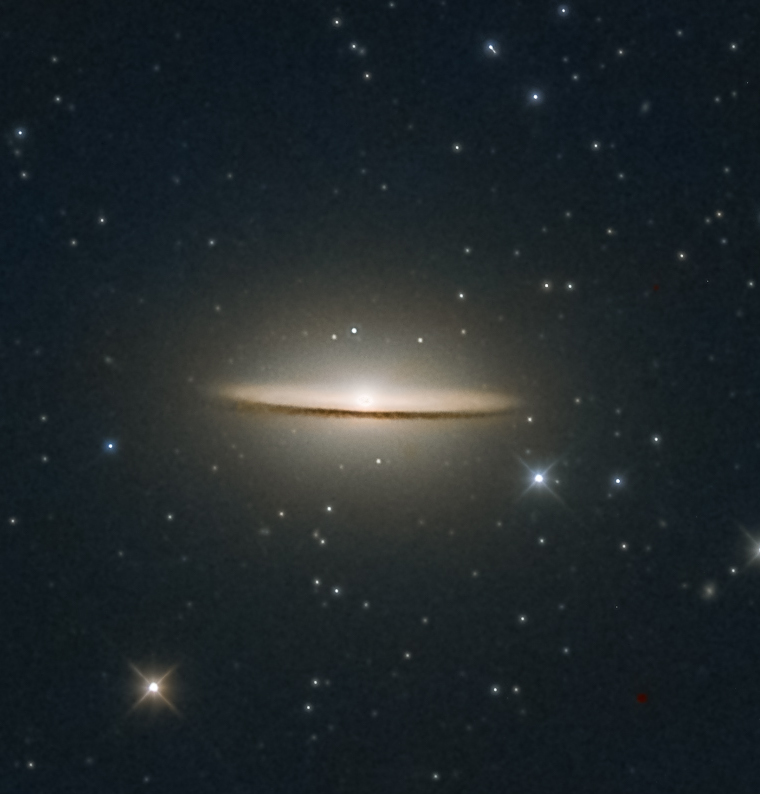
\includegraphics[height=5cm]{figures/gal3.jpg}
	\caption{The almost edge-on sombrero galaxy.\\
	Inclination angle $i \approx 90^\circ$\\Image credit:\\Carsten Frenzl}
	\end{subfigure}
\end{figure}


\item \question{Galactic Rotation curves}\\
Calculate the radial velocities from the measured wavelengths and plot them over the distance from the galaxy center. use $\lambda_0 = 21.106\,$\AA\, and 1\,pc = $3.1\cdot 10^{16}$ m.
\begin{table}[h]
\centering
\begin{tabular}{c|c|c}
$\lambda$ in \,\AA &Radius $R$ in Mpc& $v_{\text{rotation}}$ in $\frac{km}{s}$\\\hline
21.1195&1& \\
21.1130&2&\\
21.1173&5&\\
21.1194&7&\\
21.1201&10&\\
21.1208&15&\\
21.1211&20&\\
21.1215&22&\\
21.1213&25&\\
\end{tabular}
\end{table}

\item \question{Circular obits}\\
Derive for circular orbits the formula for the velocity $v$ in dependence of the distance $r$. Assume a radially symmetric mass distribution.
\item \question{Velocity of planets}\\
Assuming circular orbits, compute the velocities of the planets in our solar system. Plot the resulting rotation curve $v$ over $r$.
\item \question{Expected Rotation curve}\\
Formulate an expectation for the rotation curve of the Milky Way, assuming the mass in the bulge to be $1.6\cdot 10^{10}\,\text{M}_\odot$ and the disk to be $4\cdot 10^{10}\,\text{M}_\odot$
\item \question{Observed rotation curve}
The observed rotation curves of spiral galaxies are of the following form:
\begin{figure}[h]
	\centering
	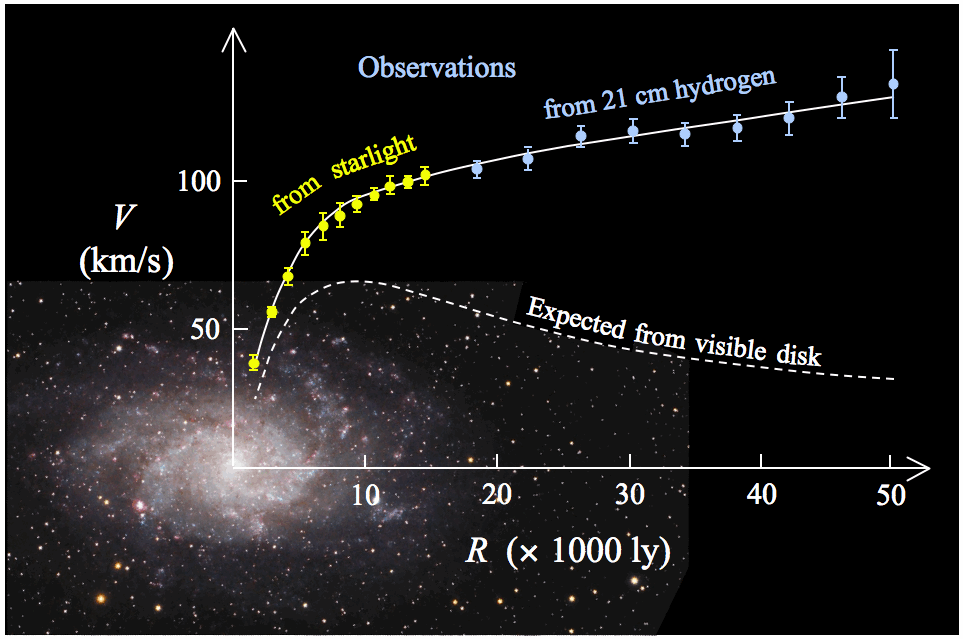
\includegraphics[width=0.5\textwidth]{figures/rotationcurve.png}
	\caption{Expected and observed rotation curve of M33.\\Image credit: Steffania Deluca}
\end{figure}
This cannot be explained by visible mass alone. Assuming that dark matter is the source of the difference between the observed and the predicted rotation curves, please calculate the mass of the dark matter depending on the velocities $v(r)$ and $v_{\text{axis}}(r)$
\item \question{Dark matter distribution}
To find out how dark matter is distributed throughout a spiral galaxy, please consider a simple rotation curve consisting of a linear and a constant branch. Assume a spherically symmetric mass distribution of the form 
\begin{equation*}
\mu(r) \propto r^k
\end{equation*}
For the mass use the formula
\begin{equation*}
M(r) = 4\pi\int_{r_0}^{r}\mu(\rho)\,\rho^2 \text{d}\rho
\end{equation*}
	\begin{enumerate}
	\item Please calculate the mass of the bulge in dependence of $k$
	\item Using the formula for $v$ from Task 3 and the result from a), please determine the exponent $k$ for the bulge. Calculate the mass of the bulge in dependence of $r$ and the complete mass $M_B$ of the bulge.
	\item To determine $k$ for the halo ($v=$ const.), consider the total mass to be composed of the mass of the bulge $M_B$ and the mass of the halo $M_H$.
	\begin{equation*}
		M(r) = M_B +M_H(r)
	\end{equation*}
	Calculate the mass outside of the bulge with the integral for the mass. Determine the exponent $k$ using the results of b) and Task 3. Find a formula for the mass of the halo in dependence of $r$.
	\item Compare the rotation curve of the bulge to the rotation curve of a rigid body.
	\end{enumerate}
\end{enumerate}
\end{document}


